\chapter{Controlling Laplacian Eigenfluids}
Many real world applications require us to optimize for some parameters of
a physics-based problem. A toy problem would be to optimize for some initial
angle and velocity of a projectile to hit some target \todo{Refer back to the
learning to throw example}. As a more involved example, \cite{MinDrag} address
finding the best shape of a vehicle to minimize its drag. These kinds of
inverse problems have been around for quite some time in engineering
applications.

Building on all of the previously introduced ideas, we now introduce our
investigation into the use of eigenfluids in fluid control problems, making use
of their explicit closed form description of a velocity field (\todo{link to
equation}). Our main proposition is to achieve reduced-order modeling-like
speed-increase: in lieu of representing the fluid as a grid, we reconstruct the
velocity field only at discrete points in space, while simulating the dynamics
of the fluid in a reduced dimensional space.\todo{Link to eq.}

\section{Our Experiments}
In the following, we showcase different optimization scenarios, where we try out
different aspects of controlling eigenfluids via \acf{DP} gradients. (See
section~\ref{dp-loss}.)

The first couple of examples are "traditional" optimization scenarios. By
"traditional", we mean finding individual solutions to problems via some
optimization technique -- in our case, \acf{GD}. Moving further, we look for
generalized solutions to a set of problems by training \acfp{NN}.

We implemented all of our experiments in $\Phi_{Flow}$
(\cite{holl2019pdecontrol}).

\subsection{Matching Velocities}\label{section:matching-velocities}
To verify the feasibility of our technique before moving on to more involved
setups, our most straightforward optimziation scenario is finding an initial
basis coefficient vector $\vb{w}_0 \in \mathbb{R}^N$ for an eigenfluid
simulation using $N=16$ basis fields, such that when simulated for $t$ time
steps, the reconstructed $\text{reconstruct}(\vb{w}_t) = \vb{u}_t$ velocity
field will match some precalculated $\vb{u}^*: [0,\pi]\times[0,\pi] \to
\mathbb{R}^2$ target velocity field:

\begin{equation}\label{eq:match-vel-loss}
  L(\vb{w}) = \left|
  \text{reconstruct}(\mathcal{P}^{t}(\vb{w})) - \vb{u}^*
  \right|_2^2,
\end{equation}

where $\mathcal{P}^t(\vb{w}) = \mathcal{P} \circ \mathcal{P} \dots \circ
\mathcal{P}(\vb{w})$ is the physical simulation of base coefficients $\vb{w}$
(in the reduced dimension) $t$ times.

For the optimization, we initialize a $\vb{w}_{init} \in \mathbb{R}^N$
vector with random numbers (from a normal/Gaussian distribution), and run the
eigenfluid simulation for $t$ timesteps, after which, we measure the error as
given by equation~\eqref{eq:match-vel-loss}, and relying on backpropagation to
derive the necessary gradients, we use the \ac{GD} optimization method as
introduced in equations~\eqref{eq:gd-steps} to iteratively find a vector
$\vb{w}_{optim}$, yielding a low scalar loss $L(\vb{w}_{optim})$.

To be able to make some further evaluation of the end results possible, we step
an eigenfluids solver for time $t$ to precalculate the target $\vb{u}^*$
velocity field, sampled on a $32\times32$ grid. Although we call its initial
basis coefficient vector $\vb{w}^*$, note that the optimization has absolutely
zero knowledge of this, as it sees only the $32\times32\times2$ velocity values
of $\vb{u}^*$. Also, these values could have been precalculated from any other
kind of fluid simulation as well, or even just initialized randomly.

We test this setup on two scenarios, with differing the number of timesteps
simulated: first with $t=16$, and then with $t=100$.

For $t=16$ simulation steps, starting from a loss of around $400$, the first
$100$ \ac{GD} optimization steps with $\lambda=10^{-3}$ reduced the loss to
under $1.0$, while $200$ steps further decreased it to under $4*10^{-4}$, with
each further step still continuously decreasing the error. 

Naturally, this very basic method has its limits.  Optimizing for initial
coefficients based only on that when reconstructed after $100$ steps of
a non-linear simulation, and reconstructed on a $32\times32$ grid, they should
match a given velocity field proved to be a substantially harder problem, as
even a relatively small error can accumulate into major deviations over these
longer timesteps, resulting in much less stable gradients.  With using the same
learning rate, the optimization diverged almost instantly. With some tuning of
the learning rate $\lambda$ in the range of $[10^{-4}, 10^{-8}]$, we were able
to get the loss below $0.14$. (Starting from an initial loss of $320$ from the
random initialization.) 

We visualize the results of these two scenarios in
Figure~\ref{fig:matching-velocities} . It is interesting to observe that even
though the optimization had absolutely no knowledge of $\vb{w}^*$, only
a comparison with a precomputed $\vb{u^*}$ velocity field at timestep $100$, the
optimized $\vb{w}_{optim}$ vector already starts to look similar to $\vb{w}^*$.
Keep in mind that this is not guaranteed at all, as highlighted with the
\todo{link to learning to throw example}. 

Although there are a number of ways to tweak this setup, we can already verify
from these results that  the flow of the gradients is working, and is ready to
be tested in more advanced scenarios.

\begin{figure}
  \centering
  \begin{subfigure}{\textwidth}
    \centering
    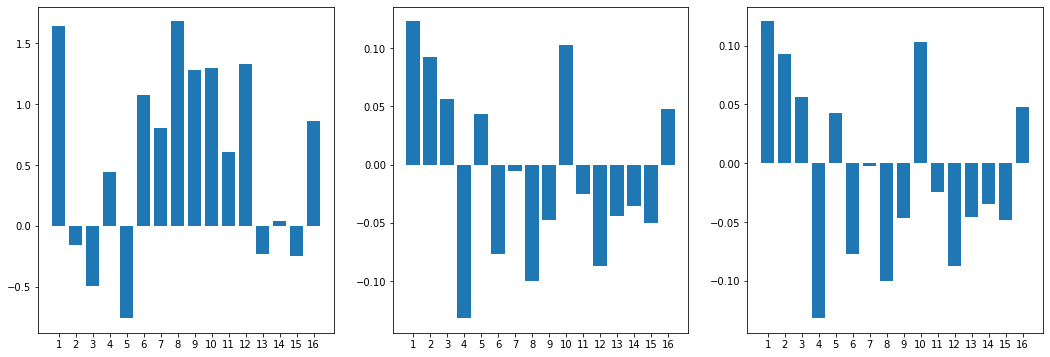
\includegraphics[width=0.9\textwidth]{figures/finding-initial-velocities/t_16_coefficients.png}
    \caption{$\vb{w}_{init}$, $\vb{w}_{optim}$, and
    $\vb{w}^*$, optimizing for velocity field after $16$ timesteps}
    \label{fig:16-timesteps-coeffs}
  \end{subfigure}\par\medskip
  \begin{subfigure}{\textwidth}
    \centering
    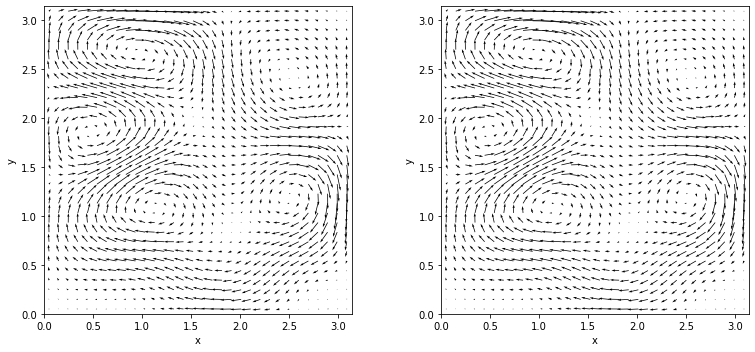
\includegraphics[width=0.8\textwidth]{figures/finding-initial-velocities/t_16_velocities.png}
    \caption{Target $\vb{u}^*$, and $\vb{u}^{16}$, reconstructed from
      $\mathcal{P}^{16}(\vb{w}_{optim})$\\}
    \label{fig:16-timesteps-vel}
  \end{subfigure}\par\medskip
  \begin{subfigure}{\textwidth}
    \centering
    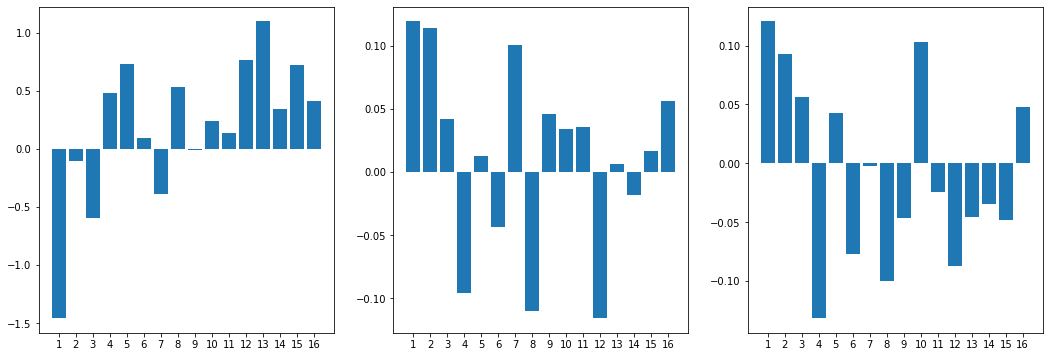
\includegraphics[width=0.9\textwidth]{figures/finding-initial-velocities/t_100_coefficients.png}
    \caption{Initial basis coefficients $\vb{w}_{init}$, $\vb{w}_{optim}$, and
    $\vb{w}^*$, optimizing for velocity field after $100$ timesteps\\}
    \label{fig:100-timesteps-coeffs}
  \end{subfigure}\par\medskip
  \begin{subfigure}{\textwidth}
    \centering
    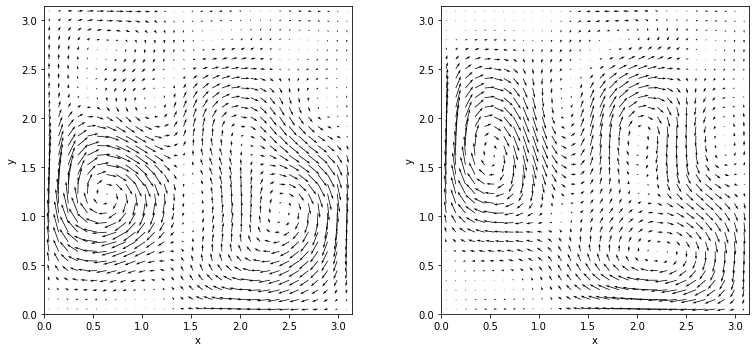
\includegraphics[width=0.8\textwidth]{figures/finding-initial-velocities/t_100_velocities.png}
    \caption{Target $\vb{u}^*$, and $\vb{u}^{100}$, reconstructed from
      $\mathcal{P}^{100}(\vb{w}_{optim})$}
    \label{fig:100-timesteps-vel}
  \end{subfigure}
  \caption{Results of optimizing for an initial $\vb{w}_0$ basis coefficient
    vector that matches a target velocity field $\vb{u}^*$ when reconstructed
    after simulating for $t$ timesteps.
  }
  \label{fig:matching-velocities}
\end{figure}

\subsection{Controlling Shape Transitions}
\label{section:controlling-shape-transitions}
In the following, we showcase an optimization scenario, with the target of
controlling the transition of two shapes in a fluid simulation setup.  The work
of \cite{holl2019pdecontrol} formulated this problem in an Eulerian
representation, with marker densities being advected by the simulated velocity
field of the fluid. 

Playing to the strength of the eigenfluids method, our experiment makes use of
its explicit formulation of the fluid velocity $\vb{u}$ as described in
section~\todo{ref section}. We stay independent of any grid resolution, and
approximating the 2D shapes via a set of sample points, we reconstruct the
velocity field only partially at a discrete set of points as needed for the
advection of these particles. This results in both a faster fluid simulation as
well as optimization as compared to fully simulating an $N\times N$ grid,
advecting a marker density, and backpropagating gradients of a physical
simulation with much more degrees of freedom.

We explore three different possibilities for addressing this problem. 
\begin{itemize}
  \item First, in a similar vein to the problem statemnt in
    section~\ref{section:matching-velocities}, we are looking for an initial
    coefficient vector $\vb{w}_0$ of an eigenfluids simulation, such that when
    simulated for $t$ time steps, the reconstructed velocity field will advect
    some initial points to the desired positions.
  \item Second, we optimize for some force vector $\vb{f}\in \mathbb{R}^{t\times
    N}$, such that $\vb{f}_t \in \mathbb{R}^N$ applied as external force to an
    eigenfluid simulation, it will yield the desired outcome.
  \item Third, we generalize the problem to looking for a function that exerts
    the necessary control force at time $t$, so that particles currently at
    positions $\vb{p}_t$ will end up at target positions $\vb{p}_{t+t}$ at the
    next timestep. We will formulate this third task as a \acf{Neural Network}
    agent in the form $\vb{f}(\vb{p_t}, \vb{p_{t+1}}, \vb{w}_{t}, \vb{\theta})$,
    also passing in the current basis coefficient vector $\vb{w}_t$, and
    optimizing for its parameters $\theta$ to yield the desired outcome.
\end{itemize}

Before moving on to each of these tasks, we will first go through the common
ground between the above three problems.

\todo{Finish section based on the notes below...}
\begin{itemize}
  \item $N=16$ basis fields
  \item the reconstructed velocity field will advect a set of initial points
$\vb{p}_0 = [p^0_0\dots p^i_0]$ to line up with target positions 
$\vb{p}_{t} = [p_t^0\dots p_t^i]$
  \item We can write this optimization problem as 
$$\arg\min_{\vb{w}} \text{Loss}(\vb{w}, \vb{p}^0, \vb{p}^t)
= \arg\min_{\vb{w}} \left| \mathcal{P}^{t}(\vb{p}^0, \vb{w})
- \vb{p}^t\right|_2^2 = \arg\min_{\vb{w}}
\sum_{i}\left|\mathcal{P}^{t}(p^0_i, \vb{w}) - p^t_i\right|_2^2, $$
where $\mathcal{P}^t(\vb{w}, \vb{p}) = \underbrace{\mathcal{P} \circ
\mathcal{P} \dots \circ \mathcal{P}(\vb{w}, \vb{p})}_{t \text{ times}}$
denotes the physical simulation of base coefficients $\vb{w}$ and 
points $\vb{p}$ in the velocity field reconstructed from $\vb{w}$. We
use a simple mean-square error (also known as $L_2$ norm) for measuring the error.
\end{itemize}

The main difficulty of this non-linear optimization problem lies in that we have
no control over the natural flow of the fluid besides supplying an initial
$\vb{w}_0$ vector.

\subsubsection*{Sampling}

\todo{We take a quick detour to discuss some sampling strategies we tried to
optimally approximate 2D shapes.}

\todo{Write about sampling strategies of points, how shapes are defined, etc.}

\subsubsection{Initial Velocity}
\todo{Write this section properly.}
Making use of the differentiability of our physical simulator $\mathcal{P}$, and
the multivariable chain rule for deriving the gradient of the above
$\mathcal{P}^t$ function composition, we can derive its gradient with respect to
the initial coefficients: $$\frac{\partial
\mathcal{P}^t(\vb{w},\vb{p})}{\partial \vb{w}}.$$

Finally, we can simply iterate a \ac{GD} optimizer with learning rate $\lambda$
to find a (good enough) solution for our above minimization problem:

$$\vb{w}_{\text{better}} = \vb{w} - \lambda
\frac{
    \partial\text{Loss}(\vb{w}, \vb{p}_0, \vb{p}_t)
}{
    \partial \vb{w}
}$$
\subsubsection{Control Force Estimation}
\todo{Write this section.}

\subsubsection{Neural Network Training}
\todo{Write this section.}
